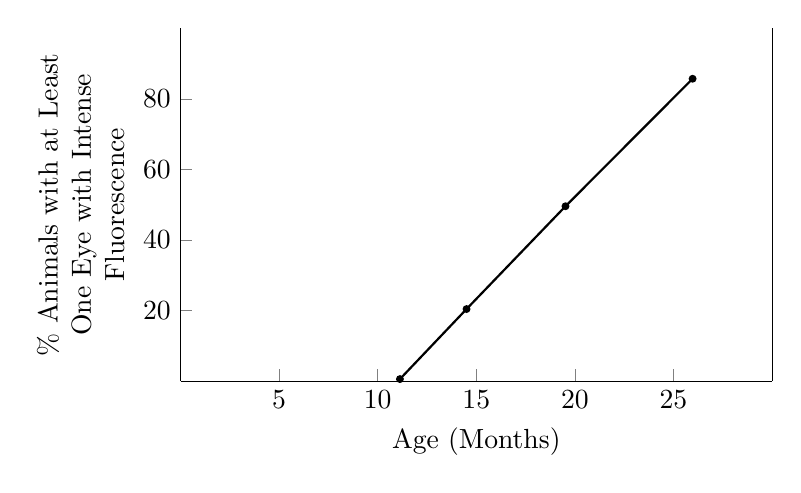
\begin{tikzpicture}
\begin{axis}[
    width=0.75\linewidth,
    height=0.5\linewidth,
    axis lines*=box,
    axis x line*=bottom,
    axis line style={-},
    xtick={5,10,15,20,25},
    ytick={20,40,60,80},
    ytick pos=left,
    xmin=0, xmax=30,
    ymin=0, ymax=100,
    ylabel={\% Animals with at Least\\One Eye with Intense\\Fluorescence},
    xlabel={Age (Months)},
    ylabel style={align=center},
    clip=false
]

\addplot[mark=*, mark size=1pt, thick] coordinates {
    (11.127879886098887, 0.5627750453016063)
    (14.505565622573128, 20.409008542583493)
    (19.524203986538957, 49.546725342997675)
    (25.970748123220297, 85.67952368625423)
};

\end{axis}
\end{tikzpicture}
